\documentclass[12pt]{article}
\usepackage{tkz-tab}
\usepackage{tikz}
\usepackage{xcolor}
\usepackage{amsmath}

\begin{document}
\begin{center}
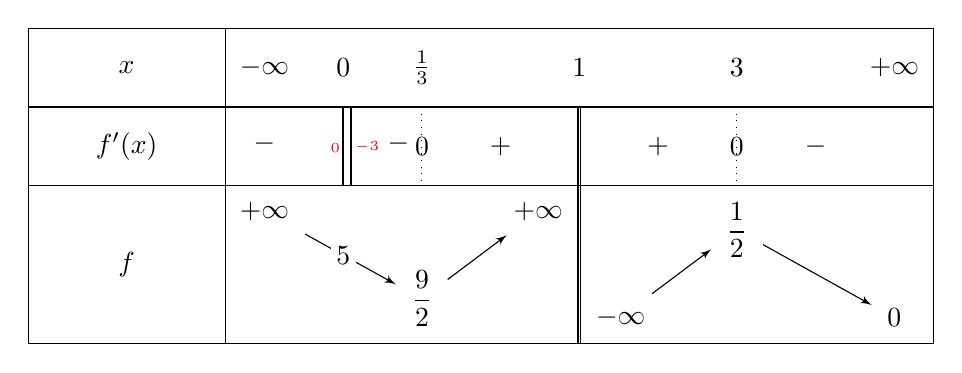
\begin{tikzpicture}
  \tkzTabInit[lgt=2.5, espcl=2]
    {$x$/1, $f'(x)$/1, $f$/2}
    {$-\infty$, $\frac{1}{3}$, $1$, $3$, $+\infty$}

  \tkzTabLine{ ,   , z , + , d , + , z , - }
  \tkzTabVar{+/$+\infty$ , -/ $\dfrac{9}{2}$ , +D-/$+\infty$/$-\infty$ , +/ $\dfrac{1}{2}$ , -/ $0$}
  \tkzTabVal{1}{2}{0.5}{$0$}{5}

  % Barres verticales à x = 0
  \draw[thick] (4.0, -2) -- ++(0, 1);
  \draw[thick] (4.1, -2) -- ++(0, 1);

	\node[above] at (3.9, -1.7) {\tiny\textcolor{red}{$0$}};
	\node[above] at (4.3, -1.7) {\tiny\textcolor{red}{$-3$}};

  	\node[above] at (3, -1.7) {\textcolor{black}{$-$}};
	\node[above] at (4.7, -1.7) {\textcolor{black}{$-$}};
\end{tikzpicture}
\end{center}
\end{document}